\chapter{Uporaba in pisanje funkcij}
\section{Kaj so funkcije in zakaj so uporabne?}
Kot že vemo, funkcije predstavljajo del kode, ki jo lahko izvedemo tako, da funkcijo preprosto pokličemo. 

Uporaba funkcij ima veliko prednosti. Govorili smo že o tem, da je glavno vodilo programiranja razdelitev problemov na obvladljive podprobleme. Določanje algoritma, ki ga potem samo še prenesemo v programsko kodo, je podobno določanju recepta, ki ga potem prenesemo v okusno jed. Prav tako, kot se moramo pri kuhanju zavedati sestavin, ki jih imamo na razpolago, se moramo tudi pri programiranju zavedati gradnikov programskega jezika, ki jih lahko pri pisanju algoritma uporabimo. 

Funkcije nam omogočajo, da osnovne korake za reševanje programa vgradimo v enostavnejše funkcije, enostavnejše funkcije v kompleksnejše in tako naprej. Podobno, kot če bi pri peki torte lahko uporabili že vnparej pripravljeno testo, preliv in kar se pri torti še uporabi, namesto da moramo torto sestaviti iz enostavnejših (nižjenivojskih) sestavin, kot so jajca, mleko in sladkor. Tako, kot bi lahko tudi pri peki seveda šli v drug ekstrem in se lotili reje kokoši, bi na veliko nižji nivo lahko šli tudi pri programiranju, ampak pustimo to za kdaj drugič. S pisanjem svojih funkcij se lahko torej najprej lotimo enostavnejših korakov, ki predstavljajo del rešitve izbranega problema. Potem lahko vmesne rešitve (velikokrat na enostaven način) združimo v končno rešitev. Če bi npr. želeli najti vsa praštevila v določenem razponu števil, bi lahko najprej napisali funkcijo, ki za podano število preveri, če je praštevilo. Vse kar bi morali narediti potem bi bil zgolj klic te funkcije za vsako število z intervala.

Zgled s praštevili pa nam je posredno razodel še eno veliko prednost uporabe funkcij. Isto kodo, tj. preverjanje ali je neko število praštevilo, bomo poklicali večkrat, vsakič seveda z drugim argumentom, tj. številom, ki je kandidat za praštevilo. Funkcije nam torej omogočajo tudi to, da lahko isti kos kode večkrat pokličemo brez tega, da bi jo vključevali v zanke ali pa kopirali v vse dele programa, kjer jo potrebujemo. 

To kodo bi lahko delili tudi z drugimi programerji. Če smo npr. napisali zelo dobro funkcijo za iskanje praštevil in smo nad njo nadvse navdušeni, hkrati pa vemo, da bi bila lahko koristna tudi za druge iskalce praštevil, lahko funkcijo enostavno zapakiramo v t.i. modul, ki ga objavimo na internetu. 

\section{Kako definiramo funkcijo?}

Vsaki funkciji, ki jo želimo v naših programih ponovno uporabiti, moramo dati seveda neko ime, preko katerega jo bomo lahko po potrebi poklicali. Skupaj s seznamom argumentov, ki jih bo naša funkcija sprejela, to podamo v definiciji funkcije. Definicijo funkcije začnemo z rezervirano besedo \texttt{def} in končamo z dvopičjem:

\begin{lstlisting}[language=Python]
def ime_funkcije(argument_1, argument_2,..., argument_n):
\end{lstlisting}

Definiciji funkcije sledi njena vsebina. Stavke, ki so v funkciji vsebovani tudi tokrat določimo z zamikanjem na začetku vrstice (podobno kot pri pogojnemu stavku in zankah). Ko želimo Pythonu sporočiti, da koda ni več del funkcije, enostavno nehamo zamikati.

Spodnji primer predstavlja definicijo enostavne funkcije, ki sešteje vrednosti dveh spremenljivk (\texttt{a} in \texttt{b}) v novo spremenljivko (\texttt{c}) in rezultat seštevanja izpiše.
\begin{lstlisting}[language=Python,numbers=left]
def sestej(a, b):
    c = a + b
    print(c)
    # tale komentar je še del funkcije
# tale komentar ni več del funkcije
\end{lstlisting}

Kaj pa se zgodi, ko program s tole definicijo poženemo. Navidez se ne zgodi nič, če pa v ukazno vrstico napišemo ime pravkar definirane funkcije, bi moral Python izpisati nekaj podobnega temu:
\begin{lstlisting}[language=Python]
<function sestej at 0x000001C24E1481E0>
\end{lstlisting}
Kaj to pomeni? To pomeni, da se je v našem \emph{imenskem prostoru} (pojem bomo razložili v kratkem) pojavilo ime \texttt{sestej}, ki ima v ozadju funkcijo, ta pa je shranjena nekje v pommnilniku (natančneje na pomnilniškem naslovu \texttt{0x000001C24E1481E0}). Ko smo izvedli zgornjo kodo, smo torej dobili definicijo funkcije \texttt{sestej}, ki jo zdaj lahko pokličemo.

Do zdaj smo funkcije vedno klicali tako, da so imenu funkcije sledili oklepaji, znotraj katerih smo našteli vrednosti argumentov, nad katerimi smo želeli funkcijo poklicati. In seveda je tako tudi v primeru funkcij, ki jih definiramo sami. Če bi torej želeli izpisati vsoto števil 5 in 7, bi lahko izvedli klic
\begin{lstlisting}[language=Python]
>>>sestej(5,7)
12
\end{lstlisting}

Ko smo funkcijo definirali se torej koda znotraj funkcije sploh ni izvedla. Izvedla se je zgolj njena definicija, ki nam je njeno ime umestila v imenski prostor (podobno, kot če smo nekemu imenu -- sprememnljivki, priredili neko vrednost). Dejanska izvedba stavkov znotraj funkcije pa se je izvršila šele, ko smo funkcijo poklicali. Mimogrede, če bi v funkciji imeli napako, kot je npr. uporaba nedefinirane spremenljivke, bi jo Python našel šele ob klicu funkcije.

\section{Globalni imenski prostor}
Vsakič, ko v Pythonu definiramo novo spremenljivko, se ime, preko katerega bomo dostopali do vrednosti te spremenljivke, shrani v t.i. \emph{imenski prostor}. Podobno se zgodi ob definiciji funkcije, le da se v tem primeru za imenom funkcije skriva vsebina funkcije, ki se bo izvedla, ko jo bomo poklicali. Ko npr. definiramo spremenljivki \texttt{x} in \texttt{y} z uporabo kode
\begin{lstlisting}[language=Python]
>>> x = 5
>>> y = 7
\end{lstlisting}
se v imenskem prostoru pojavita imeni \texttt{x} in \texttt{y}, za katerimi se skrivata podani vrednosti, kot prikazuje slika \ref{img:imenski_prostor_1}.
\begin{figure}
    
\includegraphics[width=\linewidth]{img/imenski_prostor.pdf}
    \caption{Imena v imenskem prostoru kažejo na konkretne vrednosti v pomnilniku.}
    \label{img:imenski_prostor_1}
\end{figure}
Preko imen \texttt{x} in \texttt{y} lahko zdaj dostopamo do vrednosti, ki se skrivajo v ozadju, ne da bi se morali zavedati kje konkretno v pomnilniku so te vrednosti shranjene, kar nam bistveno olajša življenje.

Definicije novih imen, pa naj gre za imena spremenljivk ali funkcij, ki jih ustvarimo izven funkcij, se shranijo v t.i. \emph{globalni imenski prostor}. Zato tem imenom pogosto rečemo kar globalna imena, spremenljivkam pa \emph{globalne spremenljivke}. Če obstaja globalni imenski prostor pa bo verjetno obstajal tudi lokalni. Poglejmo si, kaj se zgodi, ko funkcijo pokličemo.

\section{Kaj se zgodi ob klicu funkcije in lokalni imenski prostor}
Kot smo že omenili, se ob definiciji funkcije v globalnem imenskem prostoru ustvari novo ime, ki je enako imenu funkcije. To kaže na samo funkcijo, tako da bomo lahko le-to kasneje preko imena tudi poklicali. Situacijo po definiciji funkcije \texttt{sestej} prikazuje slika \ref{img:imenski_prostor_2}. \begin{figure}
    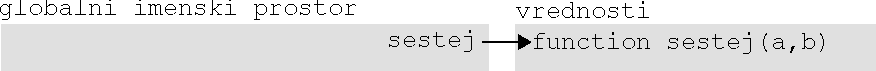
\includegraphics[width=\linewidth]{img/imenski_prostor_2.pdf}
    \caption{Ob definiciji funkcije v imenskem prostoru dobimo novo ime, ki je enako imenu funkcije. Za tem imenom se skriva naša funkcija.}
    \label{img:imenski_prostor_2}
\end{figure}

Dopolnimo program, v katerem smo napisali funkcijo \texttt{sestej}, še z njenim klicem.
\begin{lstlisting}[language=Python,numbers=left]
def sestej(a, b): # definicija funkcije
    c = a + b
    print(c)
x = 5
y = 7
sestej(x,y) # klic funkcije
\end{lstlisting}
Vrstice programa od 1, 4 in 5 bi morale biti zdaj že popolnoma jasne. Kaj pa se zgodi, ko program pride do vrstice 6? Ustvari se lokalni imenski prostor funkcije \texttt{sestej}, znotraj katerega bo funkcija ustvarila svoje lokalne spremenljivke. V lokalnem imenskem prostoru se najprej ustvarita lokalni spremenljivki z imeni \texttt{a} in \texttt{b}, ki predstavljata \emph{plitvi} kopiji spremenljivk \texttt{x} in {y}, tj. spremenljivk, s katerimi smo funkcijo poklicali. Enako posledico bi imela prireditev
\begin{lstlisting}[language=Python]
>>> a = x
>>> b = y
\end{lstlisting}
s to razliko, da bi se imeni \texttt{a} in \texttt{b} ustvarili v globalnem imenskem prostoru.

Plitva kopija pomeni, da vrednost, ki je shranjena v pomnilniku dobi dodatno ime, brez da bi se dejansko kopirala (to bi bila globoka kopija), s čimer smo s pomnilniškim prostorom veliko bolj varčni. O tem bomo še govorili, zaenkrat pa se vrnimo k naši funkciji in njenem lokalnem imenskem prostoru. Situacijo ob klicu funkcije prikazuje slika \ref{img:imenski_prostor_3}.
\begin{figure}
    \centering
    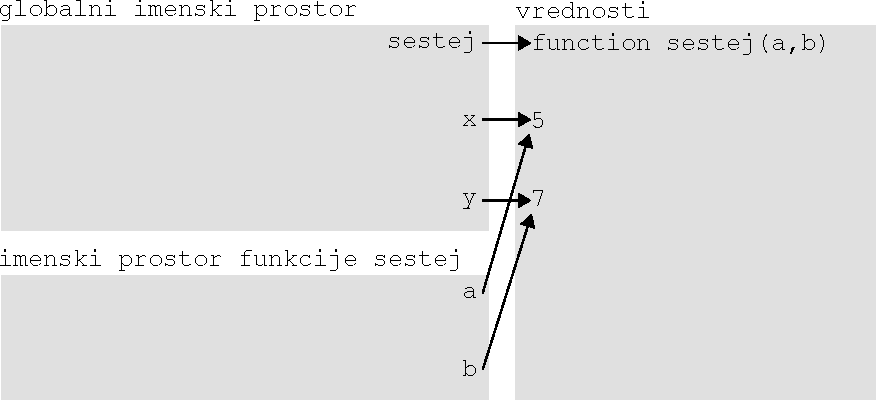
\includegraphics[width=\linewidth]{img/imenski_prostor_3.pdf}
    \caption{Ob klicu funkcije se ustvari njen lokalni imenski prostor znotraj katerega se dodatno ustvarijo plitve kopije vrednosti, s katerimi smo funkcijo poklicali.}
    \label{img:imenski_prostor_3}
\end{figure}

Vsa imena, ki jih bomo v nadaljevanju definirali znotraj funkcije, bodo ustvarjena v lokalnem imenskem prostoru funkcije. Ko naš program na primer izvede vrstico 2 (ta se je ob definiciji funkcije preskočila in se izvede šele ob njenem klicu), bo prišlo do situacije, kot jo prikazuje slika \ref{img:imenski_prostor_4}
\begin{figure}
    \centering
    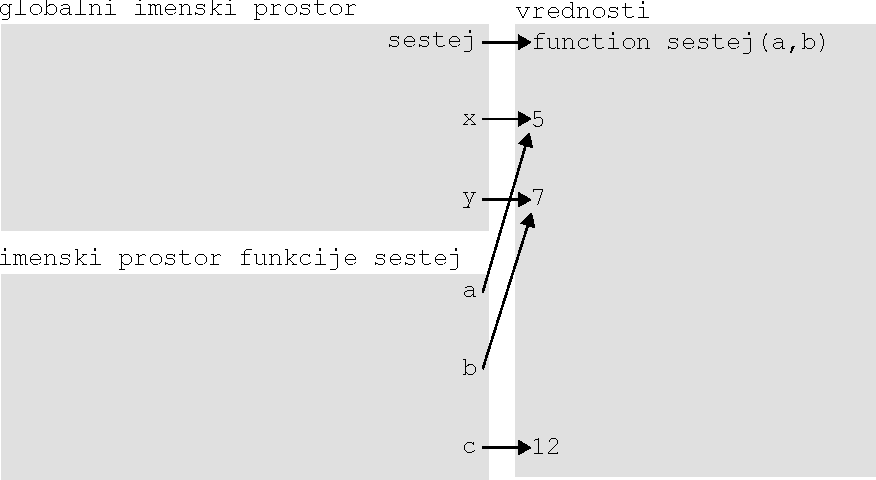
\includegraphics[width=\linewidth]{img/imenski_prostor_4.pdf}
    \caption{Vsa imena, ki jih definiramo znotraj funkcije, se ustvarijo zgolj v lokalnem imenskem prostoru te funkcije.}
    \label{img:imenski_prostor_4}
\end{figure}

Kaj pa bi se zgodilo, če bi znotraj funkcije definirali ime, ki obstaja že v globalnem imenskem prostoru. Nič posebnega. Spremenljivka s tem imenom bi se ustvarila v lokalnem imenskem prostoru funkcije in to na globalno spremenljivko ne bi vplivalo. Zgodilo bi se nekaj takega kot prikazuje slika \ref{img:imenski_prostor_5}.
\begin{figure}
    \centering
    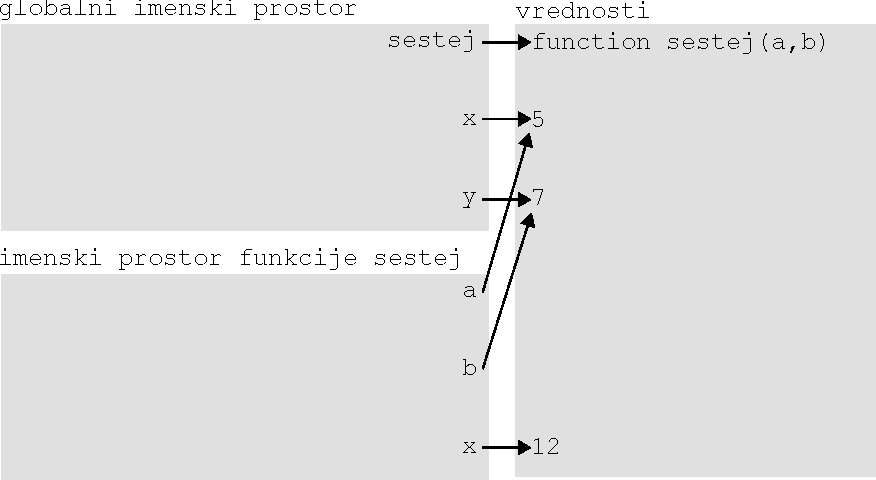
\includegraphics[width=\linewidth]{img/imenski_prostor_5.pdf}
    \caption{Znotraj funkcije lahko uporabljamo enaka imena spremenljivk kot izven funkcije in s tem ne vplivamo na globalne spremenljivke.}
    \label{img:imenski_prostor_5}
\end{figure}

Zakaj je tak način delovanja dober? Če bi morali znotraj funkcij paziti, da ne uporabljamo enakih imen, kot so že definirana izven funkcij, potem bi morali že vnaprej predvideti kakšna imena bodo pri programiranju uporabljali vsi bodoči uporabniki naših funkcij. Prav tako bi morali biti zelo pazljivi, ko bi obstoječe funkcije uporabljali mi. Vedeti bi morali katere spremenljivke za izpis nečesa na zaslon na primer uporablja funkcija \texttt{print}. Tem imenom bi se morali izogibati, kar pa bi bilo skrajno nerodno in nesmiselno.

Vprašanje, na katerega moramo še odgovoriti je, kaj se zgodi, ko se funkcija izvede do konca. V našem primeru se funkcija konča po izpisu vrednosti spremenljivke \texttt{c} (vrstica 3). Ko se funkcija konča, njenega lokalnega imenskega prostora ne potrebujemo več. Če bomo funkcijo še enkrat poklicali, bo Python ustvaril nov lokalen imenski prostor. Iz tega razloga po končanju izvedbe funkcije lokalni imenski prostor funkcije izgine. V našem konkretnem primeru torej imena \texttt{a}, \texttt{b} in \texttt{c} izginejo. Kaj pa vrednosti? Do vrednosti 12 ne moremo več dostopati preko nobene spremenljivke, zato se lahko izbriše tudi ta. Vrednosti 5 in 7 po drugi strani ostaneta, saj nanju še vedno kažeta imeni \texttt{x} in \texttt{y}. To prikazuje slika \ref{img:imenski_prostor_6}.
\begin{figure}
    \centering
    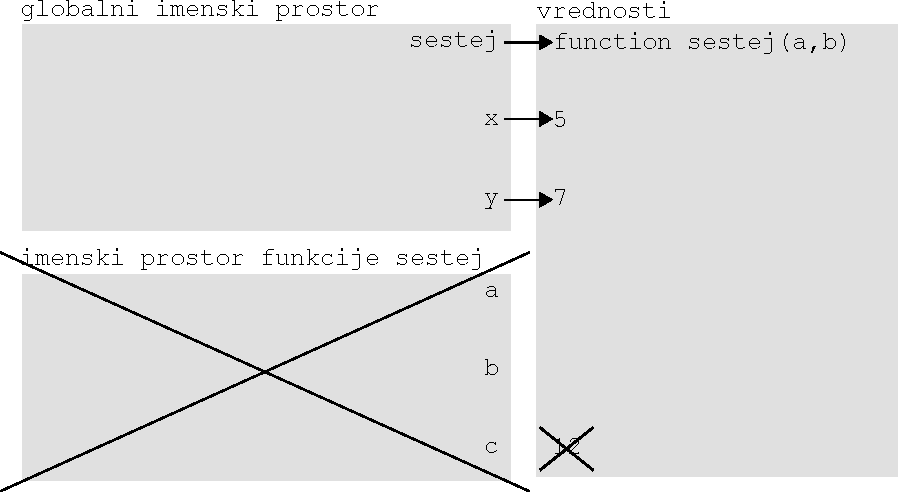
\includegraphics[width=\linewidth]{img/imenski_prostor_6.pdf}
    \caption{Po izvedbi klica funkcije, se njen imenski prostor izbriše.}
    \label{img:imenski_prostor_6}
\end{figure}

Iz globalnega imenskega prostora do lokalnih imenskih prostorov uporabljenih funkcij torej ne moremo dostopati, saj se po zaključku izvajanja funkcij (ko izvedba programa preide spet v globalni imenski prostor), lokalni imenski prostori izbrišejo. Kaj pa obratno? Iz lokalnega imenskega prostora funkcije, lahko dostopamo do globalnega (tudi zato se mu reče globalni), kar pomeni, da lahko dostopamo do vrednosti globalnih spremenljivk. Še pomembneje pa je to, da lahko iz lokalnega imenskega prostora funkcij, dostopamo do imen globalno definiranih funkcij. To pomeni, da lahko iz posamezne funkcije pokličemo druge funkcije (gnezdenje funkcij) ali pa tudi samo sebe. Slednjemu se reče \emph{rekurzija}, ampak pustimo to za kdaj drugič. 

Napišimo malo razširjen program, ki bo seštel vrednosti dveh seznamov. Pri tem si bomo pomagali z definicijo dveh funkcij.
\begin{lstlisting}[language=Python,numbers=left]
def sestej(a, b): # seštej in izpiši
    c = a + b
    print(c)

def sestej_seznama(a,b): # seštej istoležne elemente
    for i in range(len(a)):
        sestej(a[i], b[i])

sestej_seznama([1,2,3],[4,5,6]) # klic funkcije
\end{lstlisting}
Iz funkcije \texttt{sestej\_seznama} torej kličemo funkcijo \texttt{sestej}. Ali je to dovoljeno? Seveda. Imeni \texttt{sestej} in \texttt{sestej\_seznama} bomo po izvedbi vrstic 1 in 5 imeli v globalnem imenskem prostoru, kot prikazuje slika  \ref{img:imenski_prostor_7}.
\begin{figure}
    \centering
    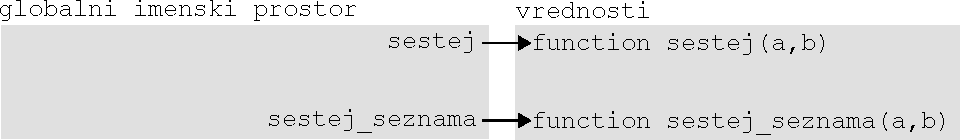
\includegraphics[width=\linewidth]{img/imenski_prostor_7.pdf}
    \caption{Imeni definiranih funkcij sta shranjeni v globalnem imenskem prostoru, zato jih lahko pokličemo od kjerkoli.}
    \label{img:imenski_prostor_7}
\end{figure}

Ker je globalni imenski prostor viden tudi iz lokalnih imenskih prostorov posameznih funkcij, jih lahko od tam tudi pokličemo. V sled temu je zgornji program popolnoma pravilen. 

Če program pogledamo podrobneje, lahko vidimo, da obe funkciji uporabljata enaka imena spremenljivk. Tudi to ne bo povzročalo nobenih težav, saj bo vsaka funkcija dobila svoj lasten lokalni imenski prostor. Ko bomo poklicali funkcijo \texttt{sestej\_seznama}, bo ta dobila lokalen imenski prostor. Ko bomo iz te funkcije poklicali funkcijo \texttt{sestej}, bo ta dobila svoj imenski prostor, ki se s prostorom funkcije \texttt{sestej\_seznama} ne bo prekrival. Lokalne imenske prostore si torej lahko predstavljamo kot ločene mehurčke, ki se med seboj ne prekrivajo. Stanje našega programa ob prvi izvedbi funkcije \texttt{sestej} do vključno vrstice 2 prikazuje slika \ref{img:imenski_prostor_8}.
\begin{figure}
    \centering
    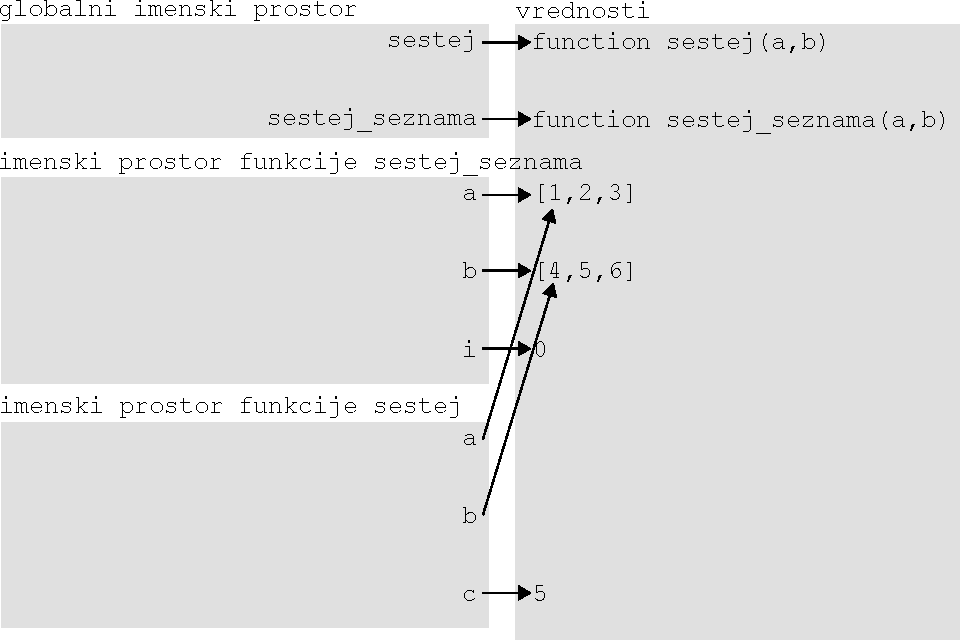
\includegraphics[width=\linewidth]{img/imenski_prostor_8.pdf}
    \caption{Lokalni imenski prostori funkcij so med seboj ločeni.}
    \label{img:imenski_prostor_8}
\end{figure}

Vprašanje za razmislek -- zakaj se znotraj funkcije \texttt{sestej} ne ustvarita novi vrednosti, na kateri bosta kazali imeni \texttt{a} in \texttt{b}?

\section{Vsaka funkcija vrača rezultat}
V splošnem pri programiranju ločimo dva tipa funkcij, in sicer tiste, ki nekaj uporabnega vrnejo in tiste, ki nekaj uporabnega naredijo (vrnejo pa nič). V določenih programskih jezikih ti dve skupini nosijo celo posebna imena in sta tudi drugače definirani. Kaj pa v jeziku Python? V skupino funkcij, ki nekaj uporabnega vračajo bi lahko uvrstili npr. funkcijo \texttt{input}, ki prebere uporabnikov vnos in tega vrne kot podatkovni tip \texttt{str}. V skupino funkcijo, ki ne vračajo nič kaj preveč uporabnega, je pa uporabno tisto, kar naredijo, pa spada funkcija \texttt{print}. Dejstvo je, da v Pythonu vsaka funkcija nekaj vrne pa tudi, če to ni čisto nič uporabnega. Poglejmo si kaj vrne funkcija \texttt{print}. Kako? Rezultat funkcije \texttt{print} bomo shranili v spremenljivko in vrednost te spremenljivke izpisali.
\begin{lstlisting}[language=Python]
>>>a = print("testni izpis")
testni izpis
>>>print(a)
None
\end{lstlisting}
Kaj se torej skriva v rezultatu funkcije \texttt{print}? Dobesedno nič oziroma \texttt{None}. Funkcija nekaj vrne, in sicer vrne nič. Preverimo lahko tudi njegov podatkovni tip.
\begin{lstlisting}[language=Python]
>>>print(type(a))
<class 'NoneType'>
\end{lstlisting}
Nič oziroma \texttt{None} je torej poseben podatek, ki pripada podatkovnemu tipu nič oziroma \texttt{NoneType}. Ni sicer veliko, ampak nekaj pa je. Enak rezultat vračajo funkcije, ki smo jih definirali v prejšnjem razdelku. Lahko preverite sami.

Kaj pa če bi želeli, da naša funkcija vrne nekaj uporabnega? V tem primeru moramo od nje to eksplicitno zahtevati, in sicer s stavkom \texttt{return}.

Spremenimo funkcijo \texttt{sestej}, tako da bo vsoto dveh števil vračala in ne izpisovala.
\begin{lstlisting}[language=Python,numbers=left]
def sestej(a, b): # seštej in vrni
    c = a + b
    return c
\end{lstlisting}
Z uporabo stavka \texttt{return} smo torej povedali, da želimo, da naša funkcija vrne vrednost spremenljivke \texttt{c}. Ali nismo tega naredili že prej? Ne. V prejšnji različici je funkcija vrednost spremenjivke \texttt{c} zgolj izpisovala. Ko se je funkcija končala, je njen lokalni imenski prostor izginil in z njim tudi vrednost spremenljivke \texttt{c}. Pogosto pa želimo rezultate funkcij uporabiti tudi v drugih delih naših programov (npr. ko uporabljamo funkcijo \texttt{input} želimo z uporabnikovim vnosom ponavadi nekaj uporabnega narediti in ga ne zgolj izpisati na zaslon). To lahko dosežemo s stavkom \texttt{return}. Kaj se zgodi, če funkcijo v našem programu zdaj še pokličemo. Razširimo program na sledeč način.
\begin{lstlisting}[language=Python,numbers=left]
def sestej(a, b): # seštej in vrni
    c = a + b
    return c
sestej(4,5)
\end{lstlisting}
Program tokrat ne izpiše ničesar. Zakaj ne? Ker tega od njega nismo nikjer zahtevali. Kaj torej naredi klic funkcije \texttt{sestej}. V konkretnem primeru nič uporabnega, saj izračuna vsoto števil 4 in 5, rezultat shrani v spremenljivko \texttt{c} in ko se funkcija zaključi, le-ta izgine, saj nanj ne kaže nobeno ime več. Kako pa bi lahko dobljeno vrednost uporabili še kje druge v našem programu? Podobno kot pri uporabi funkcije \texttt{input} -- tako, da bi rezultat funkcije priredili spremenljivki.
\begin{lstlisting}[language=Python,numbers=left]
def sestej(a, b): # seštej in vrni
    c = a + b
    return c
rezultat = sestej(4,5)
print(rezultat)
\end{lstlisting}
V zgornjem primeru bomo rezultat izpisali, lahko pa bi z njim naredili tudi karkoli drugega.

% zgled prastevila

Stavek \texttt{return} ima dvojno vlogo. Ob njegovem klicu funkcija vrne rezultat, poleg tega pa se njeno izvajanje prekine (podobno, kot če uporabimo stavek \texttt{break} v kombinaciji z zanko \texttt{while} ali \texttt{for}).

Povadimo zdaj to na iskanju praštevil. Najprej poskusimo napisati funkcijo, ki uporabniku informacijo o tem, ali število je praštevilo ali ne, zgolj izpiše.

\begin{zgled}
Napiši funkcijo, ki kot argument prejme celo število in izpiše, če je podano število praštevilo ali ne.
\end{zgled}

\begin{resitev}
Število je praštevilo, če tega ne deli nobeno od njega manjše naravno število, ki je večje od 1. Sprehoditi se moramo torej čez interval od 2 do našega števila -- 1 in za vsako število iz intervala preveriti, če deli naše število. Če na intervalu najdemo vsaj enega delitelja, število ni praštevilo in lahko iskanje takoj prekinemo. Če delitelja na celotnem intervalu ne najdemo, lahko sklepamo, da je število praštevilo.
\begin{lstlisting}[language=Python,numbers=left]
def prastevilo(stevilo):
    for i in range(2,stevilo): # razpon preiskovanja
        if stevilo % i == 0: # delitelj?
            print(stevilo, "ni praštevilo")
            break # dovolj je, da najdemo enega delitelja
    else: # če se je zanka odvrtela do konca
        print(stevilo, "je praštevilo")   
\end{lstlisting}
\end{resitev}
Poskusimo zdaj funkcijo spremeniti, tako da ne bo ničesar izpisovala, ampak bo uporabniku podala povratno informacijo o tem, če je število praštevilo ali ne.
\begin{zgled}
Napiši funkcijo, ki kot argument prejme celo število in \textbf{vrne} vrednost \texttt{True}, če je to število praštevilo, sicer pa \textbf{vrne} vrednost \texttt{False}.
\end{zgled}
\begin{resitev} \  
\begin{lstlisting}[language=Python,numbers=left]
def prastevilo(stevilo):
    for i in range(2,stevilo): # razpon preiskovanja
        if stevilo % i == 0:
            return False # prekine funkcijo in vrne False
    return True # for se je odvrtel do konca
\end{lstlisting}
\end{resitev}
Ta rešitev je bistveno lepša in enostavnejša. Iz nje vidimo dodatno prednost stavka \texttt{return}, ki poleg vračanja rezultata prekine izvajanje funkcije. Ko smo v zanki \texttt{for} našli prvega delitelja, smo prekinili izvajanje funkcije in vrnili rezultat \texttt{False}. S prekinitvijo izvajanja funkcije se je prekinila tudi zanka, zato \texttt{break} ni več potreben. Če je program prišel do vrstice številka 5, zagotovo nismo našli nobenega delitelja, saj bi sicer funkcija že vrnila \texttt{False} in se nehala izvajati. Zato lahko v vrstici 5 brezpogojno vrnemo vrednost \texttt{True}. Tako tukaj ne potrebujemo niti stavka \texttt{if}.

Dodatna prednost te rešitve je tudi to, da lahko zdaj rezultat preverjanja uporabimo tudi kje drugje. Lahko na primer napišemo funkcijo, ki izpiše vsa praštevila v določenem razponu.
\begin{zgled}
Napiši funkcijo, ki kot argument prejme celo število in izpiše vsa praštevila do vključno podanega števila.
\end{zgled}
\begin{resitev}
Vse kar je potrebno narediti, je sprehod čez interval števil od 2 do podanega števila, klic in preverjanje rezultata klica funkcije, ki smo jo definirali zgoraj.
\begin{lstlisting}[language=Python,numbers=left]
def prastevila(stevilo):
    for kandidat in range(2,stevilo+1): # kandidati
        if prastevilo(kandidat): # ali je praštevilo
            print(kandidat)
\end{lstlisting}
\end{resitev}
Rešitev je izjemno enostavna. Sprehodili smo se čez vse možne kandidate za praštevila in za vsakega preverili, če je praštevilo. Kako? Tako, da smo poklicali funkcijo, ki vrne \texttt{True}, če je podano število praštevilo. Klic te funkcije smo vstavili v stavek \texttt{if}, ki je izpisal število v primeru izpolnjenosti pogoja.

\section{Izbirni argumenti}
Včasih želimo, da imajo določeni argumenti funkcije svoje vrednosti že vnaprej določene (privzete vrednosti), razen v primeru, da želi uporabnik za te argumente uporabiti druge vrednosti. Če torej uporabnik vrednosti argumentov ne bo podal, bodo uporabljene njihove privzete vrednosti. V nasprotnem primeru bodo uporabljene uporabnikove vrednosti. Tak primer uporabe funkcij smo srečali že pri funkciji \texttt{print}, ki ima kar nekaj izbirnih argumentov. Privzeto gre funkcija \texttt{print} po vsakem klicu v novo vrstico (argument \texttt{end} je privzeto enak znaku za novo vrstico -- \texttt{\textbackslash n}), v primeru več podanih vrednosti pa te izpišejo tako, da se med njih vrine presledke (argument \texttt{sep} je privzeto enak presledku). Njune privzete vrednosti lahko povozimo, tako da jih specificiramo ob klicu, npr. kot
\begin{lstlisting}[language=Python]
>>> print(1,2,3,sep='+',end=' ')
1+2+3
\end{lstlisting}
Podobno lahko specificiramo izbirne argumente in njihove vrednosti pri definiciji svojih funkcij. 
\begin{lstlisting}[language=Python]
def ime_funkcije(arg1, arg2,..., opc1=v1, opc2=v2,...):
\end{lstlisting}
Paziti moramo samo na to, da so tisti argumenti, ki nimajo privzetih vrednosti vedno podani pred tistimi, ki privzete vrednosti imajo.

Povadimo to na malo bolj splošnem Fibonaccijevem zaporedju. Najprej poskusimo brez uporabe opcijskih argumentov.
\begin{zgled}
Napiši funkcijo, ki vrne Fibonaccijevo zaporedje števil, pri čemer naj uporabik poda dolžino zaporedja in prvi dve števili v zaporedju.
\end{zgled}
\begin{resitev}
Fibonaccijevo zaporedje je zaporedje števil, v katerem sta prva dva člena enaka številu 1, vsak nadaljnji člen pa je enak vsoti prejšnjih dveh členov. V funkciji želimo generirati bolj splošno Fibonaccijevo zaporedje, ki se začne s poljubnima številoma, npr. \texttt{a} in \texttt{b}. Znotraj funkcije bomo najprej preverili, če je željena dolžina zaporedja \texttt{n} enaka 1 (v tem primeru vrnemo seznam, ki vsebuje zgolj prvo podano število \texttt{[a]}). Sicer bomo naredili seznam z obema podanima številoma (\texttt{[a,b]}). Potem bomo še \texttt{n-2}-krat izvedli zanko, v kateri bomo v seznam vsakič dodali nov element, ki bo predstavljal vsotot trenutno zadnjih dveh elementov seznama. 
\begin{lstlisting}[language=Python,numbers=left]
def fibonacci(n, a, b):
    if n == 1:
        return [a]
    f = [a,b]
    for i in range(3,n+1):
        f.append(f[-1]+f[-2])
    return f
\end{lstlisting}
\end{resitev}
V primeru, da uporabnik želi imeti zaporedje dolžine 1, funkcija vrne zaporedje z enim elementom, in sicer \texttt{a}. V nasprotnem primeru naredi začetno zaporedje z elementoma \texttt{a} in \texttt{b} in potem v zanki doda ustrezno število dodatnih elementov, ki vsakič predstavljajo vsoto zadnjih dveh elementov zaporedja. S to rešitvijo sicer ni nič narobe, je pa dejstvo to, da si kot Fibonaccijevo zaporedje ponavadi predstavljamo zaporedje števil, ki se začne z vrednostma 1, 1. Smiselno bi torej bilo, da se privzeto naše zaporedje začne s števili 1, 1, razen če uporabnik tega ne specificira drugače. 
\begin{zgled}
Napiši funkcijo, vrne Fibonaccijevo zaporedje števil, pri čemer naj uporabnik poda dolžino zaporedja. Uporabnik lahko poda tudi prvi dve števili v zaporedju, ki sta privzeto enaki 1.
\end{zgled}
\begin{resitev} Funkcijo bomo dopolnili tako, da sta argumenta \texttt{a} in \texttt{b} opcijska in da sta privzeto postavljena na vrednost 1. 
\begin{lstlisting}[language=Python,numbers=left]
def fibonacci(n, a=1, b=1):
    if n == 1:
        return [a]
    f = [a,b]
    for i in range(3,n+1):
        f.append(f[-1]+f[-2])
    return f
\end{lstlisting}
\end{resitev}
Zgornjo funkcijo lahko torej pokličemo tudi tako, da podamo samo dolžino zaporedja. V tem primeru bosta prvi dve števili v zaporedju enaki 1, 1. V primeru, da jo bomo poklicali tako, da podamo še vrednosti za argumenta \texttt{a} in \texttt{b} pa bosta za začetna elementa uporabljeni ti vrednosti.